% -*-LaTeX-*-

\documentclass{sig-alternate-10pt}

\clubpenalty=10000 
\widowpenalty = 10000
\hyphenpenalty=5000
\tolerance=1000

%\usepackage{latexsym}
\usepackage[caption=false]{subfig}
\usepackage[sort]{cite}
\usepackage[hyphens]{url}
\usepackage{lastpage}
\usepackage{array, verbatim}
\usepackage{mdwlist}
\usepackage{multirow}
\usepackage{times}

\usepackage{hyperref,zref,xkeyval,pdfcomment}
\newcommand\todo[1]{\pdfcomment{#1}}
%\newcommand\todo[1]{}

\setlength{\pdfpagewidth}{8.5in}
\setlength{\pdfpageheight}{11in}

\usepackage{ifpdf}
\usepackage{graphicx}

\graphicspath{{./figs/}}

\ifpdf
  \DeclareGraphicsExtensions{.pdf}
\else
  \DeclareGraphicsExtensions{.eps}
\fi

%\newcommand{\enote}[2]{({\bf{#1:} \it{#2}})}
\newcommand{\enote}[2]{}

\def\full{0.8\linewidth}
\def\half{0.45\linewidth}
\def\third{0.30\linewidth}

\begin{document}



\title{Adding Heterogeneity to PlanetLab}

\numberofauthors{2}
\author{
\alignauthor
Angela H. Jiang\\
\affaddr{angelajiang@u.northwestern.edu}
\alignauthor
Zachary S. Bischof\\
\affaddr{zbischof@eecs.northwestern.edu}
}


\maketitle
%******************************************************************************
\begin{abstract}

In the past decade, PlanetLab has become a popular testbed for testing
networked systems and evaluating their performance. However, due to differences
in the architecure of PlanetLab and the general Internet, results on PlanetLab
may not translate directly into performance on the general Internet.  To
provide a more accurate platform for this purpose, researchers have attempted
to improve PlanetLab's representativeness of the Internet. While answering the
question of, ``What is representative of the general Internet?'' is an on-going
topic in research, prior works have shown characteristics of these nodes to be
generally homogenous. 


While we don't know what to model PlanetLab after, increasing the heterogeneity
of PlanetLab interconnectivity would allow researchers to customize what type
of Internet they want to represent.  We therefore focus on adding heterogeneity
to PlanetLab to increase its ability to represent the Internet.  We do this by
exploiting the existing heterogeneity of university networks in the world. We
compare the network heterogeneity of existing PlanetLab nodes with the
diversity of potential sites at universities not currently hosting a PlanetLab
node.

\end{abstract}

%******************************************************************************
\section{Introduction}

PlanetLab is a testbed for researchers in computer networking and distributed
systems. Although not part of its original purpose, many researchers have
leveraged PlanetLab for conducting measurements of the Internet.  In general,
most of its nodes are hosted in university networks.\cite{banerjee:connectivity}

However, due to the nature of its design, various network aspects of PlanetLab
nodes are found to be generally homogeneous. Sites are mostly connected to high
speed research networks located in the US and Europe. This results in little
variation between sites, as they have similar bandwidth capacities and connect
through similar types of networks.

To allow PlanetLab to be a more accurate testbed for Internet systems
experimentation, researchers have attempted to make the network more
representative of the Internet. However, understading what is
``representative'' of the general Internet is itself an important question that
researchers are still working to answer. Furthermore, it may not be something
that can be answered as the Internet will continue to grow across regions and
new devices. Instead, researchers would have to decide what ``type'' of
Internet they want to measure on by selected a different set of nodes to use
for their experiment.  We therefore focus on adding heterogeneity to PlanetLab
to improve the flexibility it provides to network researchers.

To function as a PlanetLab node, a site must meet certain resource and hardware
standards. For example, the site must be a server class machine and publicly
addressable by a static IP and hostname. These requirements allow PlanetLab
nodes to be easily managed by a remote system but is usually satisfied by
machines in University networks.  Additionally, in order to use PlanetLab for
experimentation, a researcher must purchase hardware and set up their own
PlanetLab site.\cite{dischinger:satellitelab}

The combination of both these requirements as well as the system of incentives
for creating a PlanetLab site, result in the majority of PlanetLab nodes being
located in university networks. This has caused a noticeable homogeneity in
PlanetLab sites.  In this work, we show that there is heterogeneity in
university networks that is not represented in PlanetLab. The end goal of our
work is to be able to pinpoint the universities that have the most potential to
increase PlanetLab diversity based on various network metrics such as
connectivity.

Our goal is to first determine in what ways PlanetLab is homogenous. For this,
we look at number of hops, number of ASes and types of ASes traversed between
PlanetLab nodes. Next we compare potential PlanetLab sites organized by
geography, and determine in which location would nodes have a significant
impact on PlanetLab homogeneity.


%******************************************************************************
\section{Related Work} 


Previous works have attempted to measure various network qualities of PlanetLab
nodes. Banerjee et al.\cite{banerjee:connectivity} found that 85\% of hosts are
located within an interconnected network of high speed research networks, which they 
refer to as the GREN. They also found that 91\% of origin ASes are located in North 
America while 74\% are in North American research ASes. Traffic between PlanetLab nodes
traversed 80 ASes, only 8\% of the 1123 existing ASes at the time. We are therefore
motivated to measure potential heterogeneity of other sites on the GREN.

Other works have also attempted to quantify PlanetLab’s heterogeneity. Banerjee et al.
\cite{banerjee:connectivity} compared qualities of PlanetLab’s nodes on research and 
commercial networks. Dischinger et al.\cite{dischinger:satellitelab}, looked 
at how adding hosts on edge networks could affect PlanetLab. By increasing a subset of 
PlanetLab sites with 10\% worth of edge nodes, the number of AS links tripled. This 
motivates their project, which integrates edge nodes to PlanetLab’s infrastructure. Under
SatelliteLab~\cite{dischinger:satellitelab}, the university connected network
remains central to PlanetLab.  Our attempt to increase the diversity of
university hosts would only add to the heterogeneity this project achieves.

While measuring from well-connected hosts inside academic networks, Dischinger
et al.\cite{dischinger:residential} characterized residential broadband
connections by sending packet trains to end-hosts. They included measurements
such as download and upload throughput, round-trip times and jitter, packet
loss rates, queue lengths, and queue drop policies. 



%******************************************************************************
\section{Methodology}

In this section, we describe our dataset as well as the methodology of of
experiment.  Overall, this was composed of two steps, identifying universities
that could host PlanetLab nodes and conducting measurements to these new sites.

\subsection{Selection of potential sites}

First we had to create a list of potential PlanetLab sites. We considered any
university or college that is not currently hosting a PlanetLab node to be a
potential PlanetLab site. As such, we obtain a list of universities and
colleges by crawling two websites,
Wikipedia\footnote{\url{http://en.wikipedia.org/wiki/Lists_of_universities_and_colleges_by_country}}
and Universities Worldwide\footnote{\url{http://univ.cc}}. For each school that
we found on these sites, we attempted to scrape that school's homepage. Since
many universities host their own website, we use this website as an estimate
for where the PlanetLab node would be placed. All measurements to the potential
PlanetLab site are made to the address of this website. From this list, we
identified 7010 potential sites.

Some schools may not be hosting their own page, but instead use a web hosting
company. In these cases, the hosting site could still be a potential PlanetLab
site if it adds considerable heterogeneity to the network. 

\subsection{Experiment}

After we had obtain a list of potential sites, we created a slice on PlanetLab
for measurement. We added all the PlanetLab nodes that were up and running when
we set up our experiment, resulting in 694 nodes being used for our slice. We
then conducted traceroute measurements on each PlanetLab node at a rate of one
per minute. Each node measured to all 7010 potential new sites and all 694
existing PlanetLab nodes, resulting in 7704 total sites being measured at each
node. 

Then, during the analysis step, we aggregate traceroutes by their destination,
taking a single traceroute from each PlanetLab site towards the selected
target. We then analyze all traceroutes directed towards each destination by
calculating the number of hops, number of ASes on the path, and types of ASes
traversed. We then summarize each of these metrics across all traceroutes.

%******************************************************************************
\section{Results}

In this section, we present a summary of our first cut of results. We use
present two subsets of our measurements, the results of traceroutes targeted
towards existing PlanetLab nodes, and those targeting universities in South
America and Africa. In this work, we cover three different metrics in our
analysis:

\begin{enumerate}

\item \textbf{Number of hops}. Number of hops appearing before destination IP
responds (includes non-responsive hops).

\item \textbf{Number of ASes}. Number of unique ASes seen in each traceroute.

\item \textbf{Types of ASes}. The fraction of ASes of each type according to
the classification system in Dhamdhere et. al.  For each type of AS
(access/hosting provider, content provider, enterprise customer, large transit
provider, small transit provider, tier 1, eyeball) we calculate what percentage
of each AS type we see in paths to a given destination.

\end{enumerate}

In the following subsections, we present our findings for each of these
metrics.

\subsection{Number of hops}

\begin{figure}
\centering
    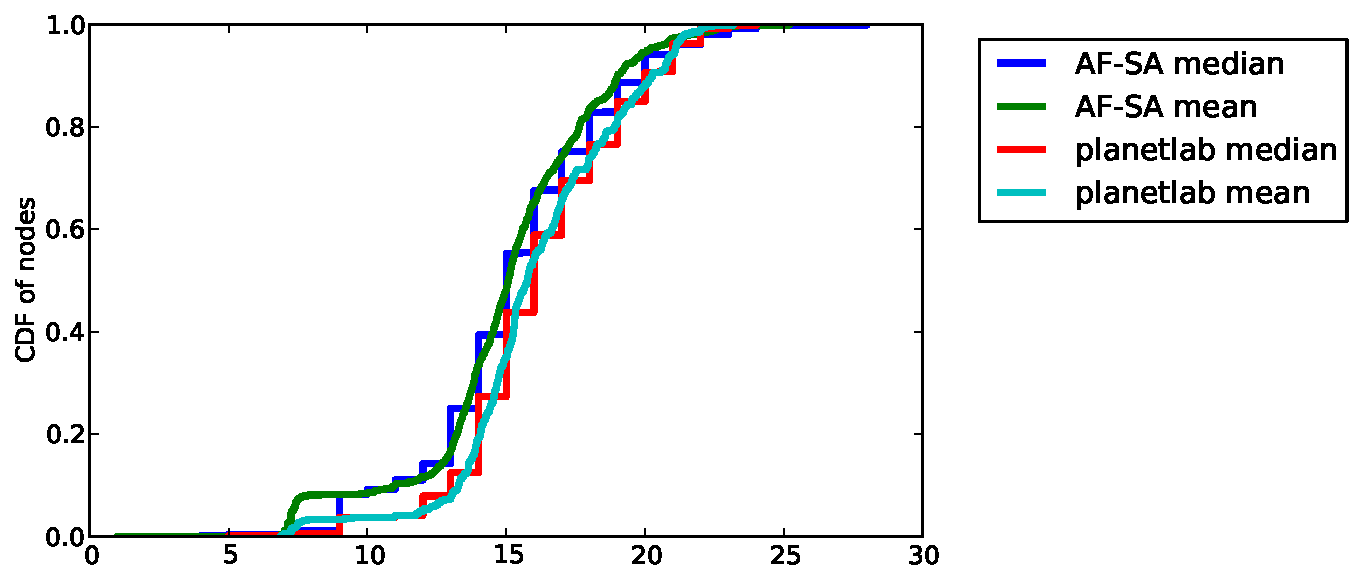
\includegraphics[width=1.0\linewidth]{figs/number_of_hops.pdf}
    \caption{Mean and median number of hops for PlanetLab and African
and South American Sites}
    \label{fig:num_hops}
\end{figure}

First we compare the number of end-to-end hops. 

\subsection{Number of AS hops}

\begin{figure}
\centering
    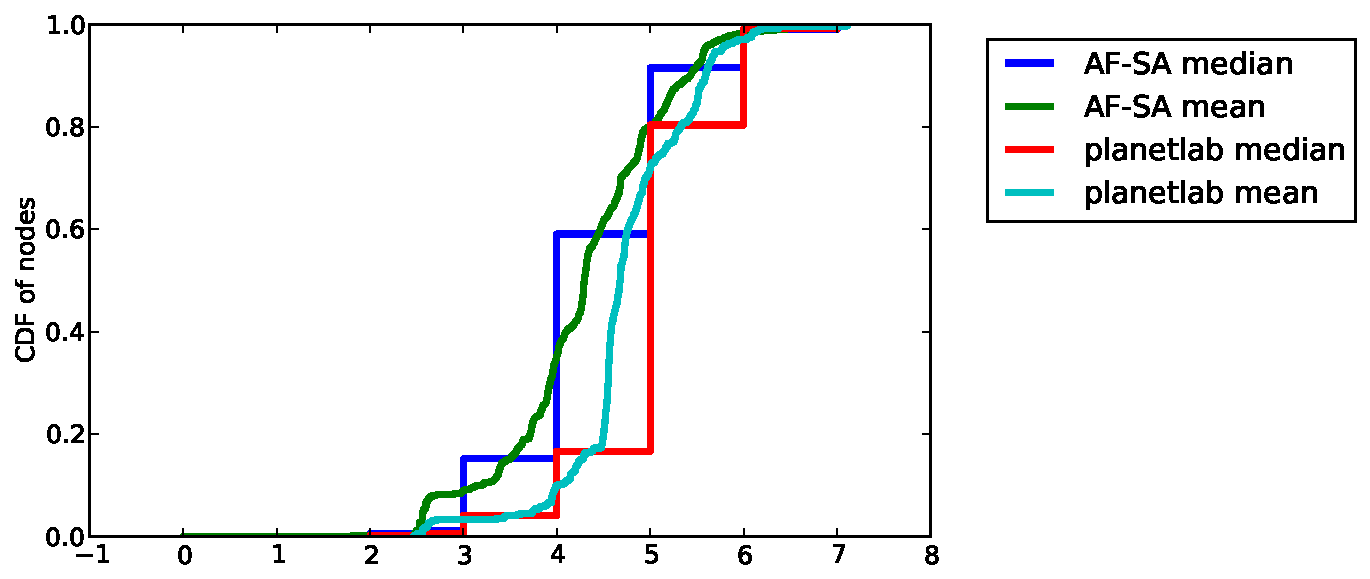
\includegraphics[width=1.0\linewidth]{figs/number_of_ases.pdf}
    \caption{Mean and median number of unique ASes for PlanetLab and African
and South American Sites}
\end{figure}

\subsection{Types of ASes}

\begin{figure}
\centering
    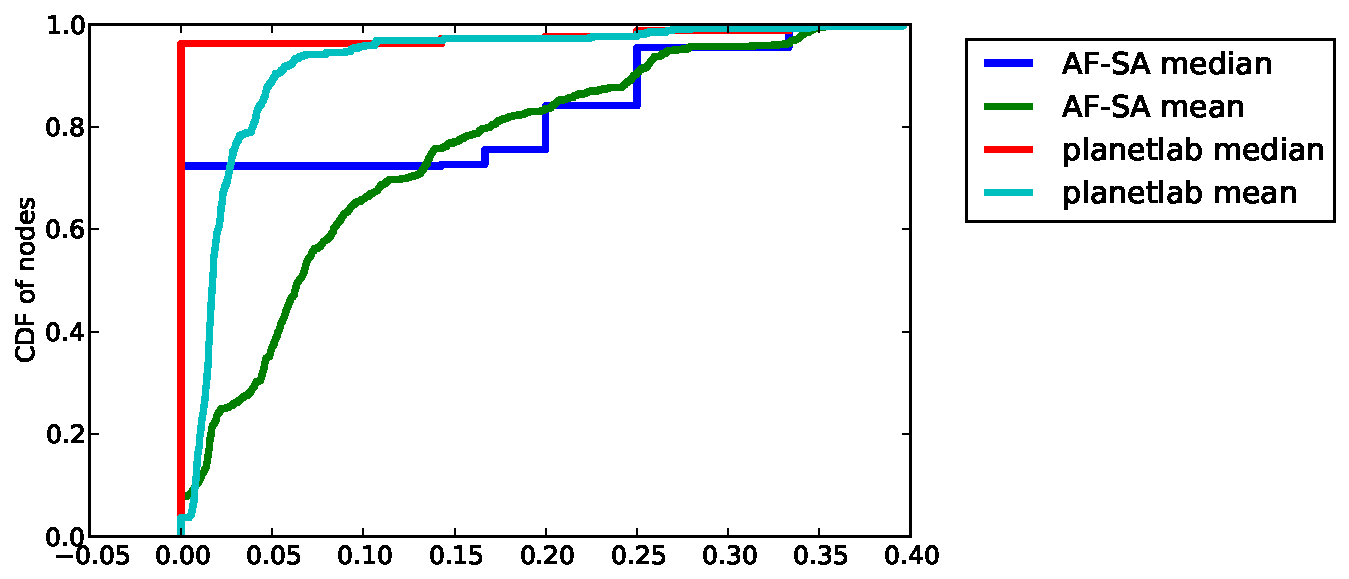
\includegraphics[width=1.0\linewidth]{figs/fractions_of_types-ltp.pdf}
    \caption{Mean and median number of unique ASes for PlanetLab and African
and South American Sites}
\end{figure}

\begin{figure}
\centering
    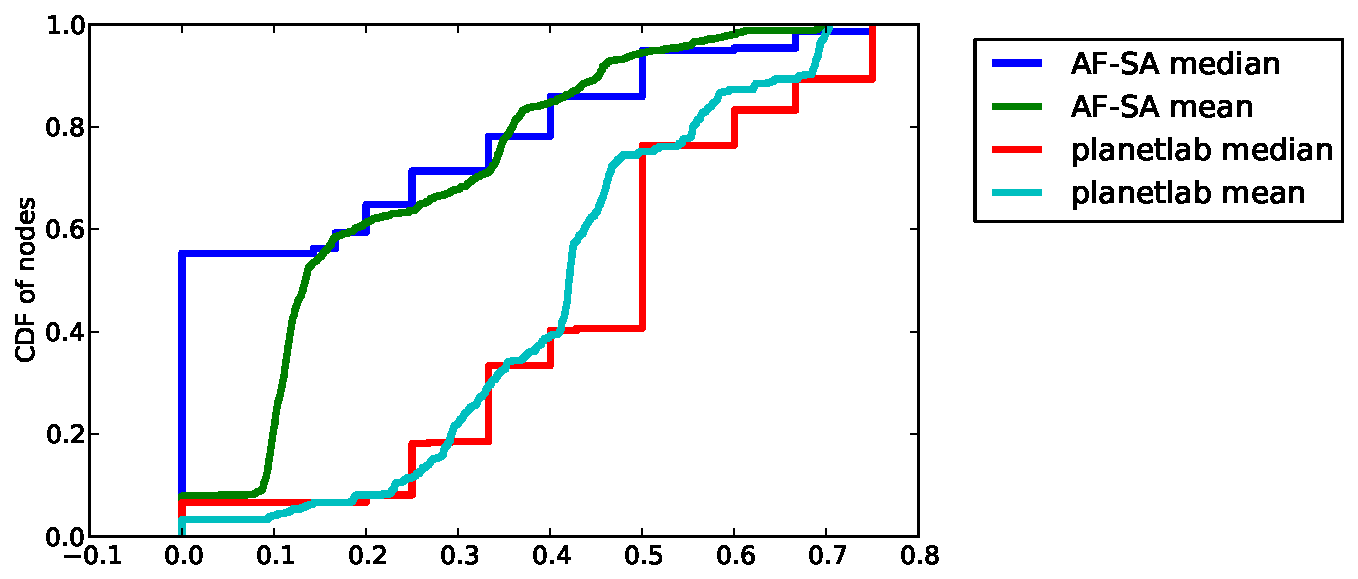
\includegraphics[width=1.0\linewidth]{figs/fractions_of_types-stp.pdf}
    \caption{Mean and median number of unique ASes for PlanetLab and African
and South American Sites}
\end{figure}

\begin{figure}
\centering
    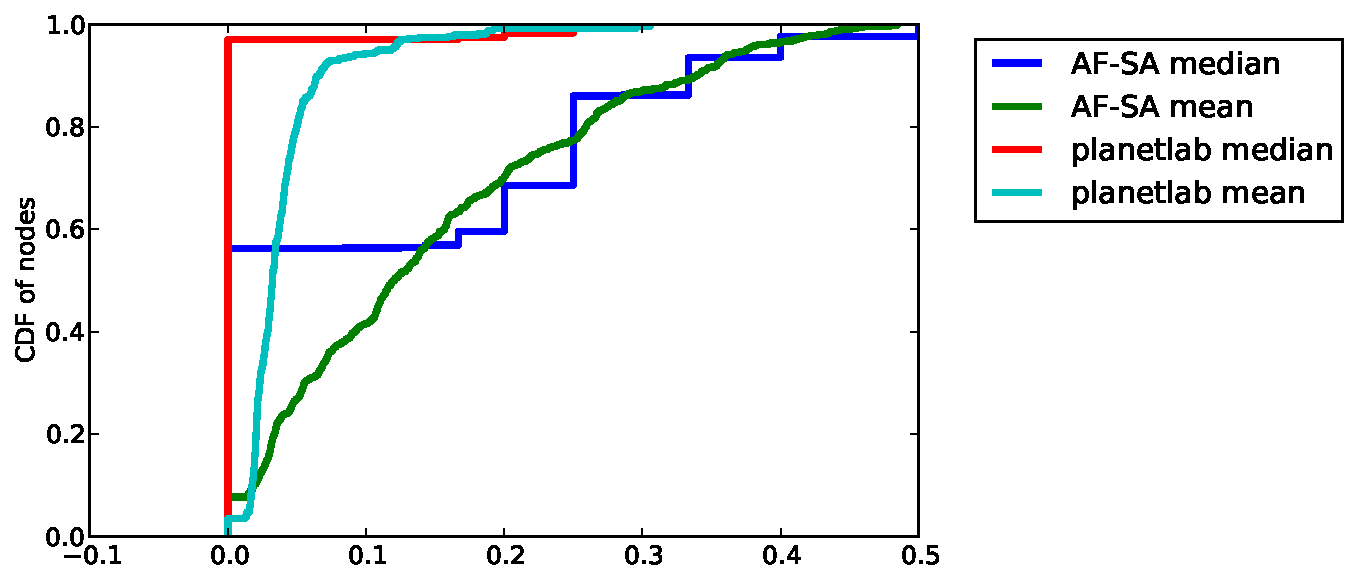
\includegraphics[width=1.0\linewidth]{figs/fractions_of_types-tier1.pdf}
    \caption{Mean and median number of unique ASes for PlanetLab and African
and South American Sites}
\end{figure}


%******************************************************************************
\section{Future work}

To continue our analysis of PlanetLab, we plan to explore more potential metrics
of heterogeneity. These include pathrate for end-to-end bandwidth measurements,
and bottleneck rates and fraction of IXP links. 

We also envision using our measurements to develop a reproducible methodology for
node selection. Selection would not be in terms of geographical location, but 
instead pinpoint sides individually. A key factor of this is determining the 
minimum number of nodes that  provide a significant impact.

%******************************************************************************
\section{Conclusion}


%******************************************************************************
\bibliographystyle{abbrv}
\bibliography{diversity}

\end{document}
